\documentclass{tufte-book}

\hypersetup{colorlinks}% uncomment this line if you prefer colored hyperlinks (e.g., for onscreen viewing)


%%
% Book metadata
\title[Workshop Artificial Life]{Workshop\\ Artificial Life}
\author[Wouter Bulten, Robert-Jan Drenth, Frank Dorssers]{Wouter Bulten, Robert-Jan Drenth, Frank Dorssers}
\publisher{Symposium committee CognAC, ACAIS 2013}

%%
% If they're installed, use Bergamo and Chantilly from www.fontsite.com.
% They're clones of Bembo and Gill Sans, respectively.
%\IfFileExists{bergamo.sty}{\usepackage[osf]{bergamo}}{}% Bembo
%\IfFileExists{chantill.sty}{\usepackage{chantill}}{}% Gill Sans

%\usepackage{microtype}

%%
% Just some sample text
\usepackage{lipsum}

%%
% For nicely typeset tabular material
\usepackage{booktabs}

%%
% For graphics / images
\usepackage{graphicx}
\setkeys{Gin}{width=\linewidth,totalheight=\textheight,keepaspectratio}
\graphicspath{{graphics/}}

% The fancyvrb package lets us customize the formatting of verbatim
% environments.  We use a slightly smaller font.
\usepackage{fancyvrb}
\fvset{fontsize=\normalsize}

%%
% Prints argument within hanging parentheses (i.e., parentheses that take
% up no horizontal space).  Useful in tabular environments.
\newcommand{\hangp}[1]{\makebox[0pt][r]{(}#1\makebox[0pt][l]{)}}

%%
% Prints an asterisk that takes up no horizontal space.
% Useful in tabular environments.
\newcommand{\hangstar}{\makebox[0pt][l]{*}}

%%
% Prints a trailing space in a smart way.
\usepackage{xspace}

%%
% Some shortcuts for Tufte's book titles.  The lowercase commands will
% produce the initials of the book title in italics.  The all-caps commands
% will print out the full title of the book in italics.

% Prints the month name (e.g., January) and the year (e.g., 2008)
\newcommand{\monthyear}{%
  \ifcase\month\or January\or February\or March\or April\or May\or June\or
  July\or August\or September\or October\or November\or
  December\fi\space\number\year
}


% Prints an epigraph and speaker in sans serif, all-caps type.
\newcommand{\openepigraph}[2]{%
  %\sffamily\fontsize{14}{16}\selectfont
  \begin{fullwidth}
  \sffamily\large
  \begin{doublespace}
  \noindent\allcaps{#1}\\% epigraph
  \noindent\allcaps{#2}% author
  \end{doublespace}
  \end{fullwidth}
}

% Inserts a blank page
\newcommand{\blankpage}{\newpage\hbox{}\thispagestyle{empty}\newpage}

\usepackage{units}

% Typesets the font size, leading, and measure in the form of 10/12x26 pc.
\newcommand{\measure}[3]{#1/#2$\times$\unit[#3]{pc}}

\usepackage{color}
\usepackage{listings}
\lstset{
	tabsize=4,
	language=matlab,
       % basicstyle=\scriptsize,
        %upquote=true,
        aboveskip={1.5\baselineskip},
        columns=fixed,
        showstringspaces=false,
        extendedchars=true,
        breaklines=true,
        prebreak = \raisebox{0ex}[0ex][0ex]{\ensuremath{\hookleftarrow}},
	frame=none,
        showtabs=false,
        showspaces=false,
        showstringspaces=false,
        identifierstyle=\ttfamily,
        keywordstyle=\color[rgb]{0,0,1},
        commentstyle=\color[rgb]{0.133,0.545,0.133},
        stringstyle=\color[rgb]{0.627,0.126,0.941},
	language=Python
}
\usepackage[parfill]{parskip}

\newcommand{\instruct}[1]{
\begin{itemize}[>]
	\item \textbf{#1}
\end{itemize}
}

\begin{document}


% r.3 full title page
\maketitle


% v.4 copyright page
\newpage
\begin{fullwidth}
~\vfill
\thispagestyle{empty}
\setlength{\parindent}{0pt}
\setlength{\parskip}{\baselineskip}
Copyright \copyright\ \the\year\ \thanklessauthor

\par\smallcaps{Published by \thanklesspublisher}


\par Licensed under the Apache License, Version 2.0 (the ``License''); you may not
use this file except in compliance with the License. You may obtain a copy
of the License at \url{http://www.apache.org/licenses/LICENSE-2.0}. Unless
required by applicable law or agreed to in writing, software distributed
under the License is distributed on an \smallcaps{``AS IS'' BASIS, WITHOUT
WARRANTIES OR CONDITIONS OF ANY KIND}, either express or implied. See the
License for the specific language governing permissions and limitations
under the License.\index{license}

\par\textit{First printing, \monthyear}
\end{fullwidth}

% r.5 contents
\tableofcontents
\setlength\parindent{0pt}
\chapter*{Introduction}
% TODO:
% -Iemand anders Mac checken of je geen paden hoeft te zetten-
% Paden hoef je dus niet te zetten mits je in de breve folder zit en vanuit daar runt
% Demo aanpassen
% Eventueel standaard paden voorstellen

The program essential to this workshop is Breve. In this guide we will be guiding you through all necessary steps to get it up and running. 

\section{Windows}
	In this section we will explain how to set up Breve under Windows.

\subsection{Installation}
	Extract the files to a location of your choosing

\subsection{Previous Python installation}
	If you have previously installed Python and added this to the path, you will have to remove the path. You can leave Python installed. If you do not remove the path, Breve will try to use the wrong Python version. Where you can find these paths can be seen in the following section.

\subsection{Setting paths}
	You will have to set two paths. One for Breve and one for the Python version that comes with Breve.

	There are two possibilities here. The first one is temporary and has to be run in command prompt every time you start a new command prompt session. It consists of the following two lines:
	\begin{verbatim}
		  set BREVE_CLASS_PATH=<breve_path>\lib\classes
		  set PYTHONPATH=\%PYTHONPATH\%;<breve_path>\lib\python2.3
	\end{verbatim}
%	\begin{lstlisting}
%		set BREVE_CLASS_PATH=<breve_path>\lib\classes
%		set PYTHONPATH=\%PYTHONPATH\%;<breve_path>\lib\python2.3
%	\end{lstlisting}
	If, for example, you have copied Breve to `C:\\breve\_2.7.2' it would look like this:
	\begin{verbatim}
		  set BREVE_CLASS_PATH=C:\breve_2.7.2\lib\classes
		  set PYTHONPATH=\%PYTHONPATH\%;C:\breve_2.7.2\lib\python2.3
	\end{verbatim}
%	\begin{lstlisting}
%		set BREVE_CLASS_PATH=C:\breve_2.7.2\lib\classes
%		set PYTHONPATH=\%PYTHONPATH\%;C:\breve_2.7.2\lib\python2.3
%	\end{lstlisting}

	There is an alternative version which is more permanent, but can easily be undone once it is not required anymore. This is done by changing the environment veriables in the Advanced System Settings:
	\begin{verbatim}
		  Ctrl+r > Fill in "control sysdm.cpl" > Press enter to run it
		  > Advanced > Environment Variables
	\end{verbatim}
%	\begin{lstlisting}
%		Ctrl+R --> Fill in "control sysdm.cpl" --> Press enter to run it --> Advanced --> Environment Variables
%	\end{lstlisting}
	% Beter alternatief vinden dan lstlisting

	Here you will see two areas, one are the user variables and the other are the system variables. We will be adding two variables to the last one. Simply press "New..." and enter the following information, substituting <breve\_path> with the actual path on your pc:
	\begin{verbatim}
		  Variable name: BREVE_CLASS_PATH
		  Variable value: <breve_path>\lib\classes
	\end{verbatim}
%	\begin{lstlisting}
%		Variable name: BREVE_CLASS_PATH
%		Variable value: <breve_path>\lib\classes
%	\end{lstlisting}
	\begin{verbatim}
		  Variable name: PYTHONPATH
		  Variable value: <breve_path>\lib\python2.3
	\end{verbatim}
%	\begin{lstlisting}
%		Variable name: PYTHONPATH
%		Variable value: <breve_path>\lib\python2.3
%	\end{lstlisting}

\subsection{Testing}
	Breve comes with several demos. You can use these to check whether the installation went okay. 

	You can run breve by running the breve executable followed by a project, don't forget to set the paths if you are using the temporary version.

	The following command prompt command will run the DLA demo:
	\begin{verbatim}
		  <breve_path>\bin\breve <breve_path>\demos\DLA.py
	\end{verbatim}
%	\begin{lstlisting}
%	<breve_path>\bin\breve <breve_path>\demos\DLA.py
%	\end{lstlisting}
	% Nog toevoegen hoe het zit als je al Python in gebruik hebt en al paden hebt ignesteld

\section{Mac OS X}
	In this section we will explain how to set up Breve under Mac OS X

\subsection{Installation}
	Extract the files to a location of your choosing.

\subsection{Setting path}
	On Mac OS X you only have to set one path. As with Windows you have two options, one is only temporary while the second is sort of permanent. 

	First of all the temporary version. Run the following line each time you start a new terminal session in which you will be using Breve:
	\begin{verbatim}
		  export BREVE_CLASS_PATH=<breve_path>/lib/classes
	\end{verbatim}
%	\begin{lstlisting}
%		export BREVE_CLASS_PATH=<breve_path>/lib/classes
%	\end{lstlisting}

	For the second, more permament version, you will have to change/create a .bash\_profile file. Anything in this file will be run each time you start a terminal session. Run the following lines in a terminal session to create or change the file:
	\begin{verbatim}
		  nano ~/.bash_profile
	\end{verbatim}
%	\begin{lstlisting}
%		nano ~/.bash_profile
%	\end{lstlisting}
	Now you have either created a .bash\_profile file or you are editing the existing version. Enter the following line:
	\begin{verbatim}
		  export BREVE_CLASS_PATH=<breve_path>/lib/classes
	\end{verbatim}
%	\begin{lstlisting}
%		export BREVE_CLASS_PATH=<breve_path>/lib/classes
%	\end{lstlisting}
	Now you can save this file by pressing `ctrl+o' and you can leave this file by pressing `ctrl+x'. After restarting the terminal you should be able to use Breve. 

\subsection{Testing}
	Breve comes with several demos. You can use these to check whether the installation went okay. 

	You can run breve by running the breve executable followed by a project, don't forget to export the path if you are using the temporary version.
	
	The following terminal command will run the DLA demo:
	\begin{verbatim}
		  <breve_path>/bin/breve <breve_path>/demos/DLA.py
	\end{verbatim}
%	\begin{lstlisting}
%	<breve_path>/bin/breve <breve_path>/demos/DLA.py
%	\end{lstlisting}
	%bin/breve demos/gatherers.tz


%%
% Start the main matter (normal chapters)
\mainmatter

\chapter{Step 1:  Creating a simulation}

Every simulation is based around a \textit{Controller} which controls the simulation. To make such a controller we extend the \textit{Breve.Control} class and implement two methods: the constructor and a iterate method.

\begin{lstlisting}[language=Python]
import breve

class SimulationController ( breve.Control ):

        def __init__( self ):
                breve.Control.__init__(self)

                print "Simulation Started"

        def iterate( self ):

                breve.Control.iterate( self )

# Start the simulation
SimulationController()
\end{lstlisting}



\instruct{Save the code above in a file called SimulationController.py.}

The \textit{\_\_init\_\_} function is called when the simulation starts and can be used to initialise other components (such as agents). 

The \textit{iterate} function is called on every iteration in the simulation. It is important to call the parent iterate method in \textit{Breve.Control}, without this the simulation will not run.

\instruct{Run the simulation to test your controller.}


\chapter{Step 2: Basic environment}
Our environment is now totally empty. To resolve this we will add a simple floor.

\instruct{In the SimulationController, add the following code in the \textit{\_\_init\_\_} function\footnote{Make sure that you place it after the call to the parent constructor.}:}

\begin{lstlisting}[language=Python]

# Create a floor for the world
self.floor = breve.Floor()
self.floor.setTextureImage(None)
            
\end{lstlisting}

These two lines add a new floor object (which has a ground plane around $Y=0$). We set the texture to None to prevent the use of the (ugly) default texture.

To improve the visual aspects of the simulation we enable lighting and shadows. This should only be used for demonstration purposes as it makes the simulation run slower.

\instruct{Add the following snippet after the code for the floor:}

\begin{lstlisting}[language=Python]
# Set display settings
self.enableLighting()
self.enableShadows()
self.moveLight(breve.vector(80,100,0))
self.enableReflections()
self.enableSmoothDrawing()
\end{lstlisting}

\chapter{Step 3: Creating an agent}
After a floor has been added we can add more objects to our world. We will start with agents.

\instruct{Create a new file agents.py}

As we are going to use functions (and classes) of the breve engine, we must import it at the top of our file.

\begin{lstlisting}[language=Python]
import breve
\end{lstlisting}

\instruct{Add the import statement to the top of our agents file.}

\section{Creating a simple agent}

We will start with a very simple agent which will do nothing but stand still. Every agent must extend the \textit{breve.Mobile} class in order for it to move and interact.

Just as with our controller, we have to add a constructor and an \textit{iterate} function.

\begin{lstlisting}[language=Python]
class SimpleAgent (breve.Mobile):

	def __init__(self):
		breve.Mobile.__init__(self)

		print "Created agent"

	def iterate(self):
		None
\end{lstlisting}

\instruct{Add the class definition above to the agents file.}

\instruct{Try to run the simulation and see what happens.}

As you can see nothing happened yet. This is because we still have to add our agent to the environment. This is done through the simulation controller.

\begin{lstlisting}[language=Python]
self.agent = agents.SimpleAgent()
\end{lstlisting}

\instruct{Add the snippet to the \textit{\_\_init\_\_} function of the controller, just below the lighting settings.}


\begin{figure}[htbp]
\begin{center}
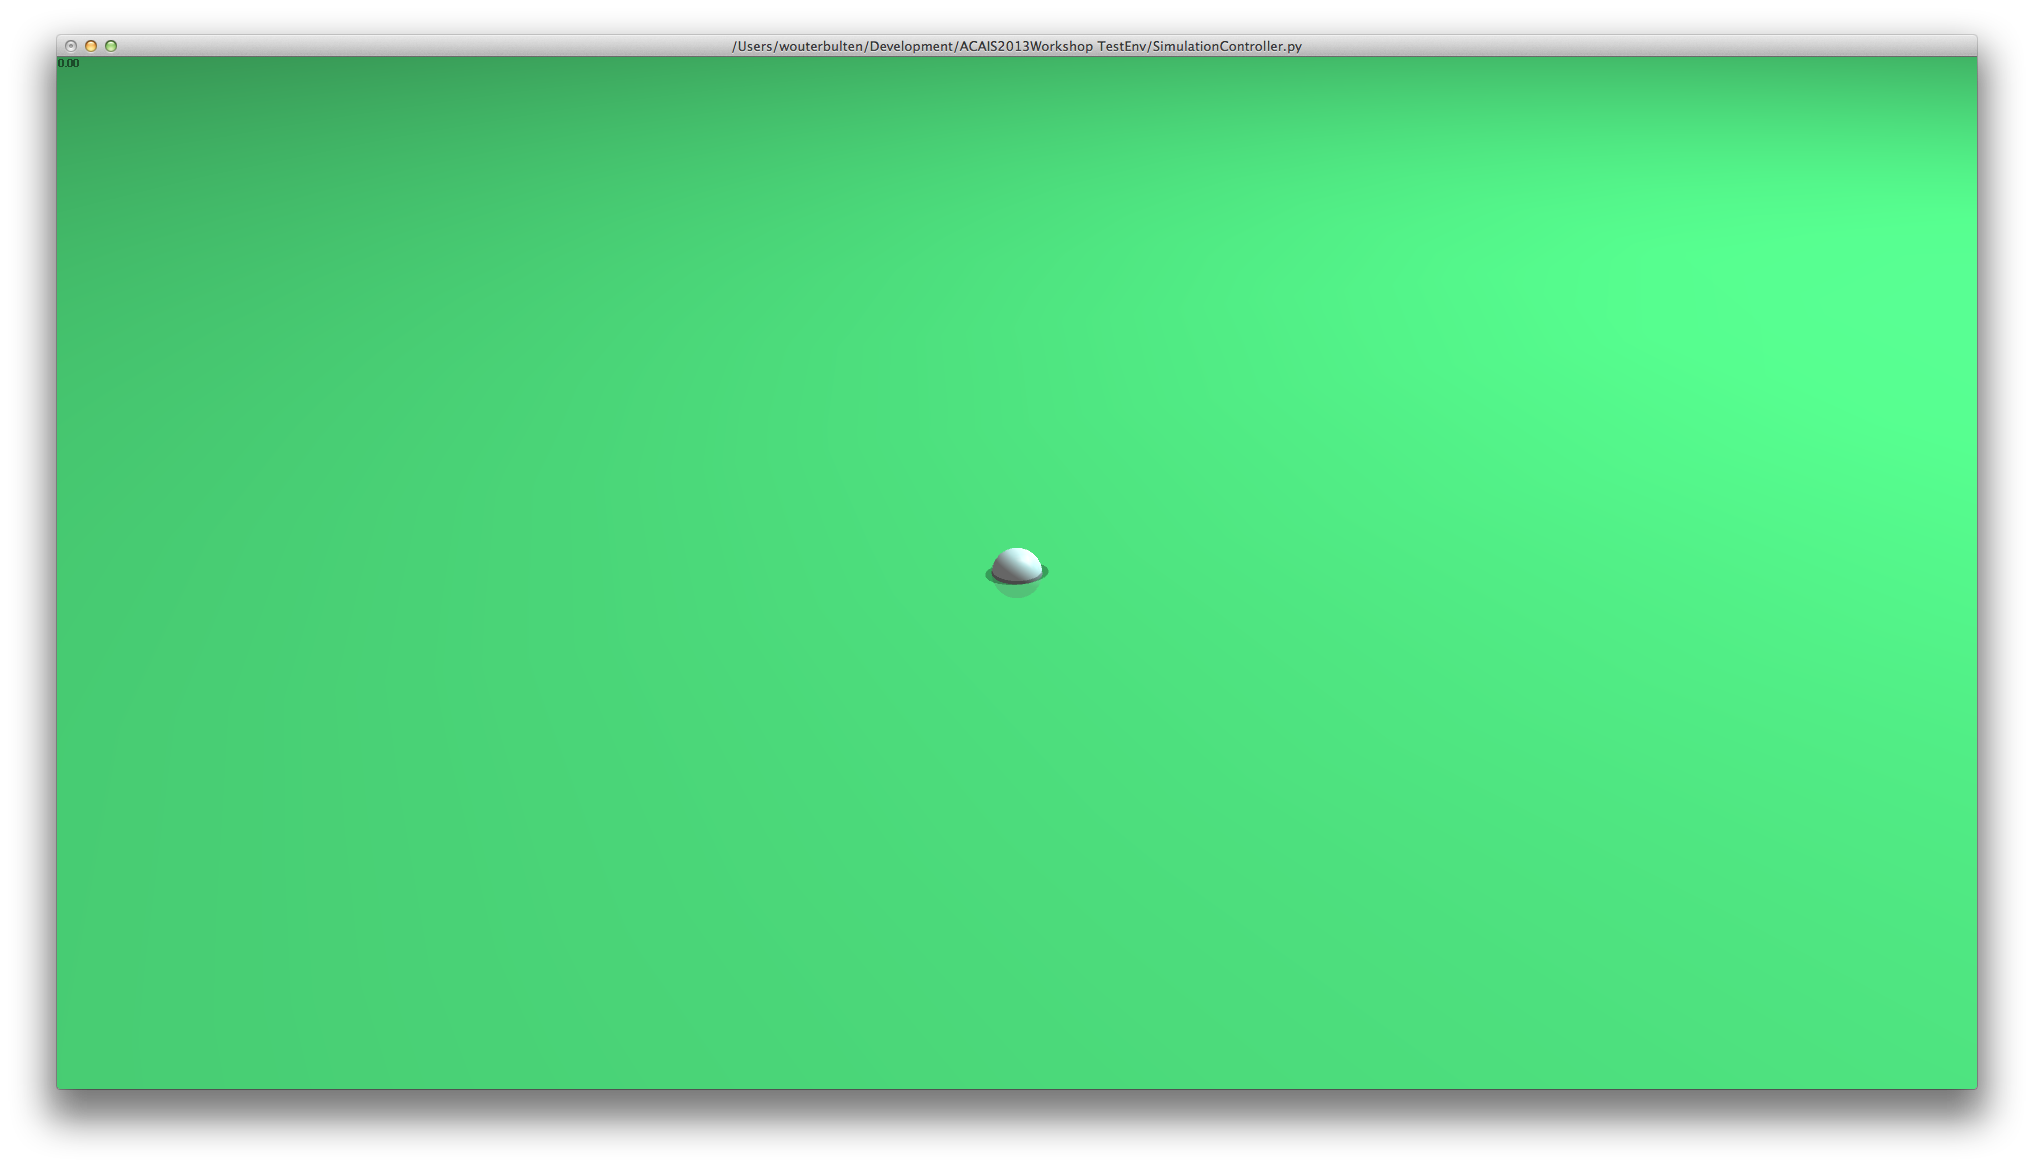
\includegraphics{graphics/simpleagent}
\caption{A single very simple agent has been added to the environment.}
\end{center}
\end{figure}

\section{Movement}
This agent is very boring, it just sits there and does nothing. We will create a new agent which wanders around in the world.

\begin{fullwidth}
\begin{lstlisting}[language=Python]
class RandomAgent (breve.Wanderer):
	def __init__(self):
		breve.Wanderer.__init__(self)

		self.setWanderRange(breve.vector(20, 0, 20))
		
		self.randomizeLocation()
		
		print "Created agent"

	def iterate(self):
		breve.Wanderer.iterate(self)
\end{lstlisting}
\end{fullwidth}

\instruct{Add the new agent class below the \textit{SimpleAgent}.}

This \textit{RandomAgent} extends the built in wanderer class of breve. The only setting we have to set is the range of the wanderer, in this case we set it to 20 in a 2D plane. It is important to call the super \textit{iterate} function, otherwise the wander behaviour will not be executed.

\instruct{Add the agent to the simulation by creating one in the constructor of the controller.}

\begin{lstlisting}[language=Python]
self.randomAgent = agents.RandomAgent()
\end{lstlisting}

\section{Appearance}

Within Breve it is very easy to change the appearance of objects and agents. As an example we are going to change the shape of our agent to a cube. As we will add more agents in the future, we will define one shape object for all agents.

\instruct{Add the following to the constructor of the SimulationController:}
\begin{fullwidth}
\begin{lstlisting}[language=Python]
# Create a shape for the agents
self.agentShape = breve.createInstances(breve.Cube, 1).initWith(breve.vector(1,1,1))
\end{lstlisting}
\end{fullwidth}

This single line will create a cube with a dimension of 1x1x1. To be able to use this shape in our agent we add a getter method to the controller.

\instruct{Add the following getter to the simulation controller:}
\begin{lstlisting}[language=Python]
def getAgentShape(self):
	return self.agentShape
\end{lstlisting}

It is now very easy to change the shape of the agent. Every \textit{Real}\footnote{The Real object is a base class for more high-level classes such as Mobile and Stationary.} object within breve has access to the simulation controller using the variable \textit{controller}. We change the shape like so:

\begin{lstlisting}[language=Python]
# Set the shape of the agent
self.setShape(self.controller.getAgentShape())
\end{lstlisting}

\instruct{Try to change the shape of the agent by adding the code to the constructor of the agent. Test it by running the simulation, has the shape changed?}

\section{Creating a group}

A single agent cannot do much. If we want to see more emergent behaviour we have to create a group. Luckily, the only thing we have to change to accomplish this is changing the way we instantiate agents. Remember that we used the following code in our controller to create a single agent:

\begin{lstlisting}[language=Python]
self.agent = agents.SimpleAgent()
\end{lstlisting}

We can now replace this with the following to create any number of agents:

\begin{lstlisting}[language=Python]
breve.createInstances(agents.RandomAgent, 10)
\end{lstlisting}

\instruct{Remove the lines that created the two agents and replace it with the snippet above. Run the simulation, you should see 10 wandering agents.}

\begin{figure}[htbp]
\begin{center}
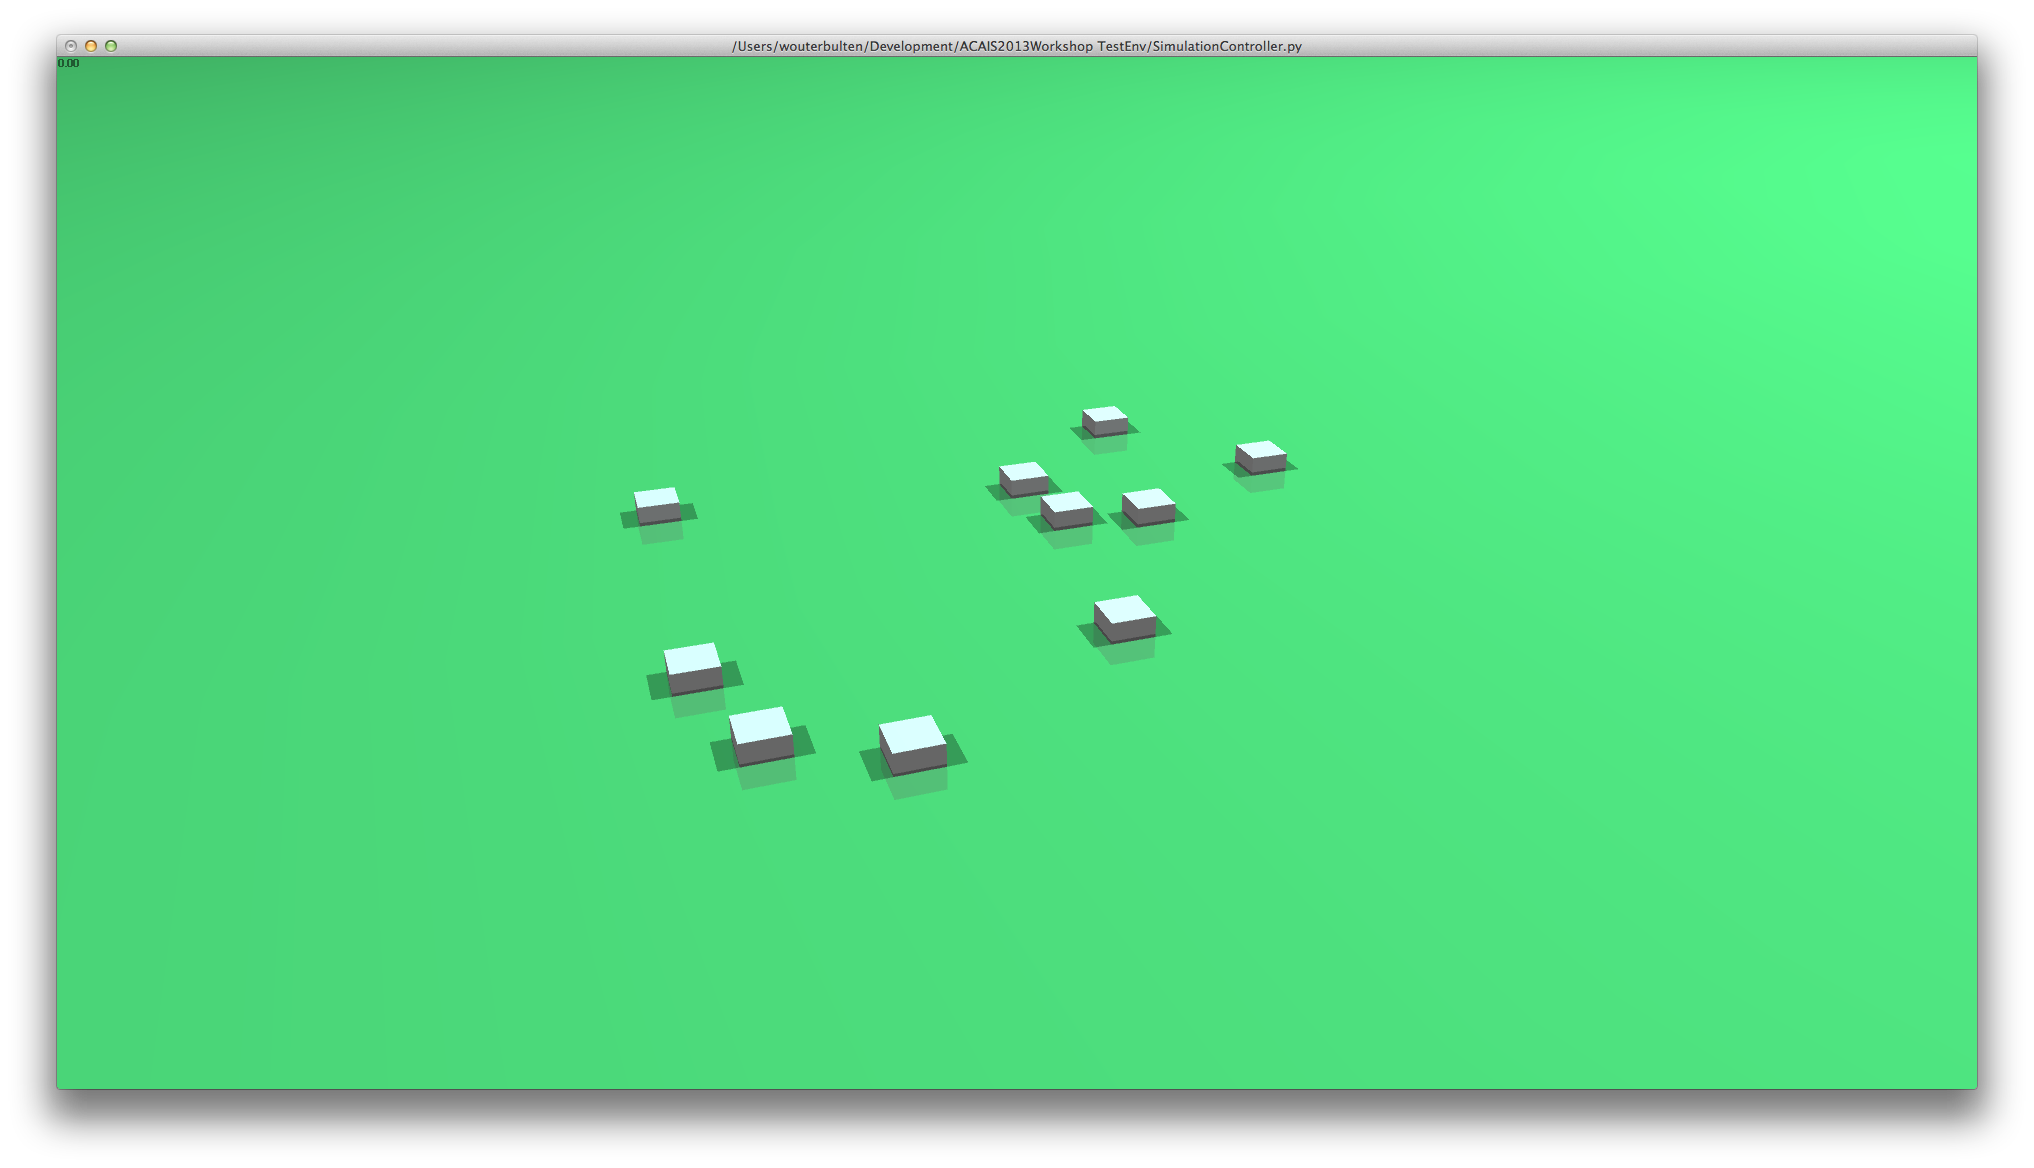
\includegraphics{graphics/randomagents}
\caption{By using the a different method of creating agents we can add multiple to the environment. In this instance 10 random agents.}
\end{center}
\end{figure}



\chapter{Step 4: Adding food}
The second object we will be adding is food. This gives our agents something that they can interact with.

\instruct{Create a new file food.py}

As we are going to use functions (and classes) of the breve engine, we must import it at the top of our file.

\begin{lstlisting}[language=Python]
import breve
\end{lstlisting}

\instruct{Add the import statement to the top of our agents file.}

\section{Creating the food object}

Our initial version of the food is very simple, it will simply stay on the field. Every food source must extend the \textit{breve.Mobile} class. Food does not have to move, but we want to be able to interact with it.

Just as with our controller and agent, we have to add a constructor and an \textit{iterate} function.

\begin{lstlisting}[language=Python]
class SimpleFood (breve.Mobile):

    def __init__(self):
        breve.Mobile.__init__(self)

    def iterate(self):
        None
\end{lstlisting}

\instruct{Add the class definition above to the agents file.}

From the previous section we know that this is not enough. We will also have to add the food to the controller

\begin{lstlisting}[language=Python]
self.SimpleFood = food.SimpleFood()
\end{lstlisting}

\instruct{Add the snippet to the \textit{\_\_init\_\_} function of the controller, just below the lighting settings.}

The food should now have been added to the simulation.

\instruct{Try to run the simulation and see what happens.}
As you can see you have now added a single food object to the field, though it does nothing yet.

\section{Location}
Our food is always at the same location when running the program. We want it to be more random. This can be done with the following function.
\begin{lstlisting}[language=Python]
def randomizedLocation(self):
    randomLoc = breve.randomExpression(2 * breve.vector(20,20,20)) - breve.vector(20,20,20)
    self.move(randomLoc)
\end{lstlisting}
\instruct{Add the function above to the food class}

Now we just have to call this function when we create the food.
\begin{lstlisting}[language=Python]
self.randomizedLocation()
\end{lstlisting}

\instruct{Add the line above to the \textit{\_\_init\_\_} function of the food}

\section{Appearance}
We will again define one shape for all food sources.

\instruct{Add the following to the constructor of the SimulationController}

\begin{lstlisting}[language=Python]
# Create a shape for the food sources
self.foodShape = breve.createInstances(breve.Sphere, 1).initWith(0.5)
\end{lstlisting}

This will create a small sphere. To be able to use this shape in our agent we add a getter method to the controller.

\instruct{Add the following getter to the simulation controller:}
\begin{lstlisting}[language=Python]
def getFoodShape(self):
    return self.foodShape
\end{lstlisting}

Now it is very easy to change the shape of the food. We change it with the following line of code:
\begin{lstlisting}[language=Python]
# Set the shape of the food source
self.setShape(self.controller.getFoodShape())
\end{lstlisting}
\instruct{Try to change the shape of the food by adding the code to the constructor of the food. Test it by running the simulation, has the shape changed?}

\section{Creating more food}
A single food object is not much for all our agents, so we want to add some more. We first added a single food object to the SimulationController with the following code:
\begin{lstlisting}[language=Python]
self.SimpleFood = food.SimpleFood()
\end{lstlisting}
We now want more food objects, this can be done with the following code:
\begin{lstlisting}[language=Python]
breve.createInstances(food.SimpleFood, 3)
\end{lstlisting}
\instruct{Replace the first piece of code with the second piece of code to create more food objects}

\chapter{Step 5: An extra dimension}
As an intermediate step, we are going to switch from a 2D plane to a 3D space to illustrate how easy it is to do so in Breve. Additionally, it will gives us a much nicer view of the final result when we get there. 

The only changes we need to make are to the \textit{agent} and \textit{food} classes; the \textit{wanderer.WanderingAgent} class which our RandomAgent extends is able to handle 2D and 3D spaces just as easily without requiring any changes in the code. 

\instruct{Change the \textit{y-value} of wander range of the RandomAgent from 0 to 20}

\begin{fullwidth}
\begin{lstlisting}[language=Python]
self.setWanderRange(breve.vector(20, 20, 20))
\end{lstlisting}
\end{fullwidth}

\instruct{Change the food.SimpleFood.randomizedLocation() function so that also a random value is taken for the y-axis}

\begin{fullwidth}
\begin{lstlisting}[language=Python]
randomLoc = breve.randomExpression(2 * breve.vector(20,20,20)) - breve.vector(20,20,20)
\end{lstlisting}
\end{fullwidth}

If you run the simulation now, you will notice how the food sources are scattered in 3D space and how the agents will move through them. As agents can now move in an area below y=0 we have to remove the floor.

\instruct{Remove the floor from the simulation controller.}

\chapter{Application: Gatherers}
\end{document}

